
	\begin{table}[H]
    \centering
		\begin{tabular}{|c|c|c||c|c|c|}
			\hline
			\rowcolor[rgb]{0.21,0.69,0.87}\multicolumn{6}{|c|}{  \textbf{ {Configuración Pines de entrada}}} \\
			\hline \hline
			\multicolumn{3}{|c|}{  \textbf{ {SensorVoy (4bits)}}} & \multicolumn{3}{|c|}{\textbf{SensorEstoy (4bits)}} \\
			\hline
			SensorVoy[0] & SW0 & F12 & SensorEstoy[0] & BTN0 & M13 \\
			\hline
			SensorVoy[1] & SW1 & G12 & SensorEstoy[1] & BTN1 & M14 \\
			\hline
			SensorVoy[2] & SW2 & H14 & SensorEstoy[2] & BTN2 & L13 \\
			\hline
			SensorVoy[3] & SW3 & H13 & SensorEstoy[3] & BTN3 & L14 \\
			\hline
		\end{tabular}
		\caption{ Configuración de los pines de entrada con las entradas del sistema }
		\label{tab:pinEntradas}
	\end{table}

	\begin{table}[H]
    \centering
		\begin{tabular}{|c|c|}
			\hline
			\rowcolor[rgb]{0.21,0.69,0.87}\multicolumn{2}{|c|}{  \textbf{ {Configuración pin CLK}}} \\
			\hline \hline
			CLK & T9 \\ 
			\hline
		\end{tabular}
		\caption{ Configuración del pin para el CLK }
		\label{tab:pinCLK}
	\end{table}

	\begin{table}[H]
    \centering
		\begin{tabular}{|c|c||c|c|c|}
			\hline
			\rowcolor[rgb]{0.21,0.69,0.87}\multicolumn{4}{|c|}{  \textbf{ {Configuración Pines de los displays de 7 segmentos}}} \\
			\hline \hline
			\multicolumn{2}{|c|}{  \textbf{ { Salida7s (7bits)}}} & \multicolumn{2}{|c|}{\textbf{Ánodos de Control}} \\
			\hline
			Salida7s[0] & E14 & Motor & AN0 & D14 \\
			\hline
			Salida7s[1] & G13 & Puerta & AN1 & G14 \\
			\hline
			Salida7s[2] & N15 & PisoVoy & AN2 & F14 \\
			\hline
			Salida7s[3] & P15 & PisoEstoy & AN3 & E13 \\
			\hline
			Salida7s[4] & R16 & - & - & - \\
			\hline
			Salida7s[5] & F13 & - & - & - \\
			\hline
			Salida7s[6] & N16 & - & - & - \\
			\hline
		\end{tabular}
		\caption{ Configuración de los pines de salida al display de 7 segmentos }
		\label{tab:pin7s}
	\end{table}
	

\subsection{Caso de Uso Práctico:}
	
	Antes de poder hacer una comprobación del funcionamiento de la maqueta debemos conocer sobre que componentes se visualizará la información:
	
	\begin{figure}[H]
        \centering
        \includegraphics[width = 0.6\textwidth ]{CasoUso/0.jpg}
        \caption{Distribución salidas/entradas de la maqueta en la Spartan-3}
        \label{fig:Spartan3Interfaz}
    \end{figure}
    
    
    \begin{itemize}
	    \item 1. Memoria 2: se ve que piso se ha guardado iluminándose el LED de dicha posición (De derecha a izquierda en orden ascendente).
	    \item 2. Memoria 1: Equivalente al anterior, refleja la posición guardada en la memoria 1.
	    \item 3. Emulan los finales de carrera para ver en qué piso se encuentra el ascensor. De derecha a izquierda en orden ascendente de pisos.
	    \item 4. Emulan los botones para seleccionar el piso al que se desea ir. De derecha a izquierda en orden ascendente de pisos.
	    \item 5. Displays para mostrar la información, se puede ver a continuación que se muestra en cada display.
	\end{itemize} 
	
	\begin{figure}[H]
        \centering
        \includegraphics[width = 0.6\textwidth ]{CasoUso/0_1.jpg}
        \caption{Distibución de las salidas a los displays}
        \label{fig:Spartan3InterfazDisplays}
    \end{figure}
    
    \begin{itemize}
		    \item  D1. Piso actual, marcado por los finales de carrera.
		    \item  D2. Piso objetivo, al que quiero ir.
		    \item  D3. Funcionamiento de la puerta.
		    \item  D4. Funcionamiento del motor.
	\end{itemize} 
	

    
	\begin{longtable}{cm{0.2\textwidth}cm{0.2\textwidth}}
	\centering
		 \includegraphics[width = 0.25\textwidth ]{CasoUso/1.jpg} & 1. &
		 \includegraphics[width = 0.25\textwidth ]{CasoUso/2.jpg} & 2.  \\
		 \includegraphics[width = 0.25\textwidth ]{CasoUso/3.jpg} & 3. & 
		  \includegraphics[width = 0.25\textwidth ]{CasoUso/4.jpg} & 4.  \\
		 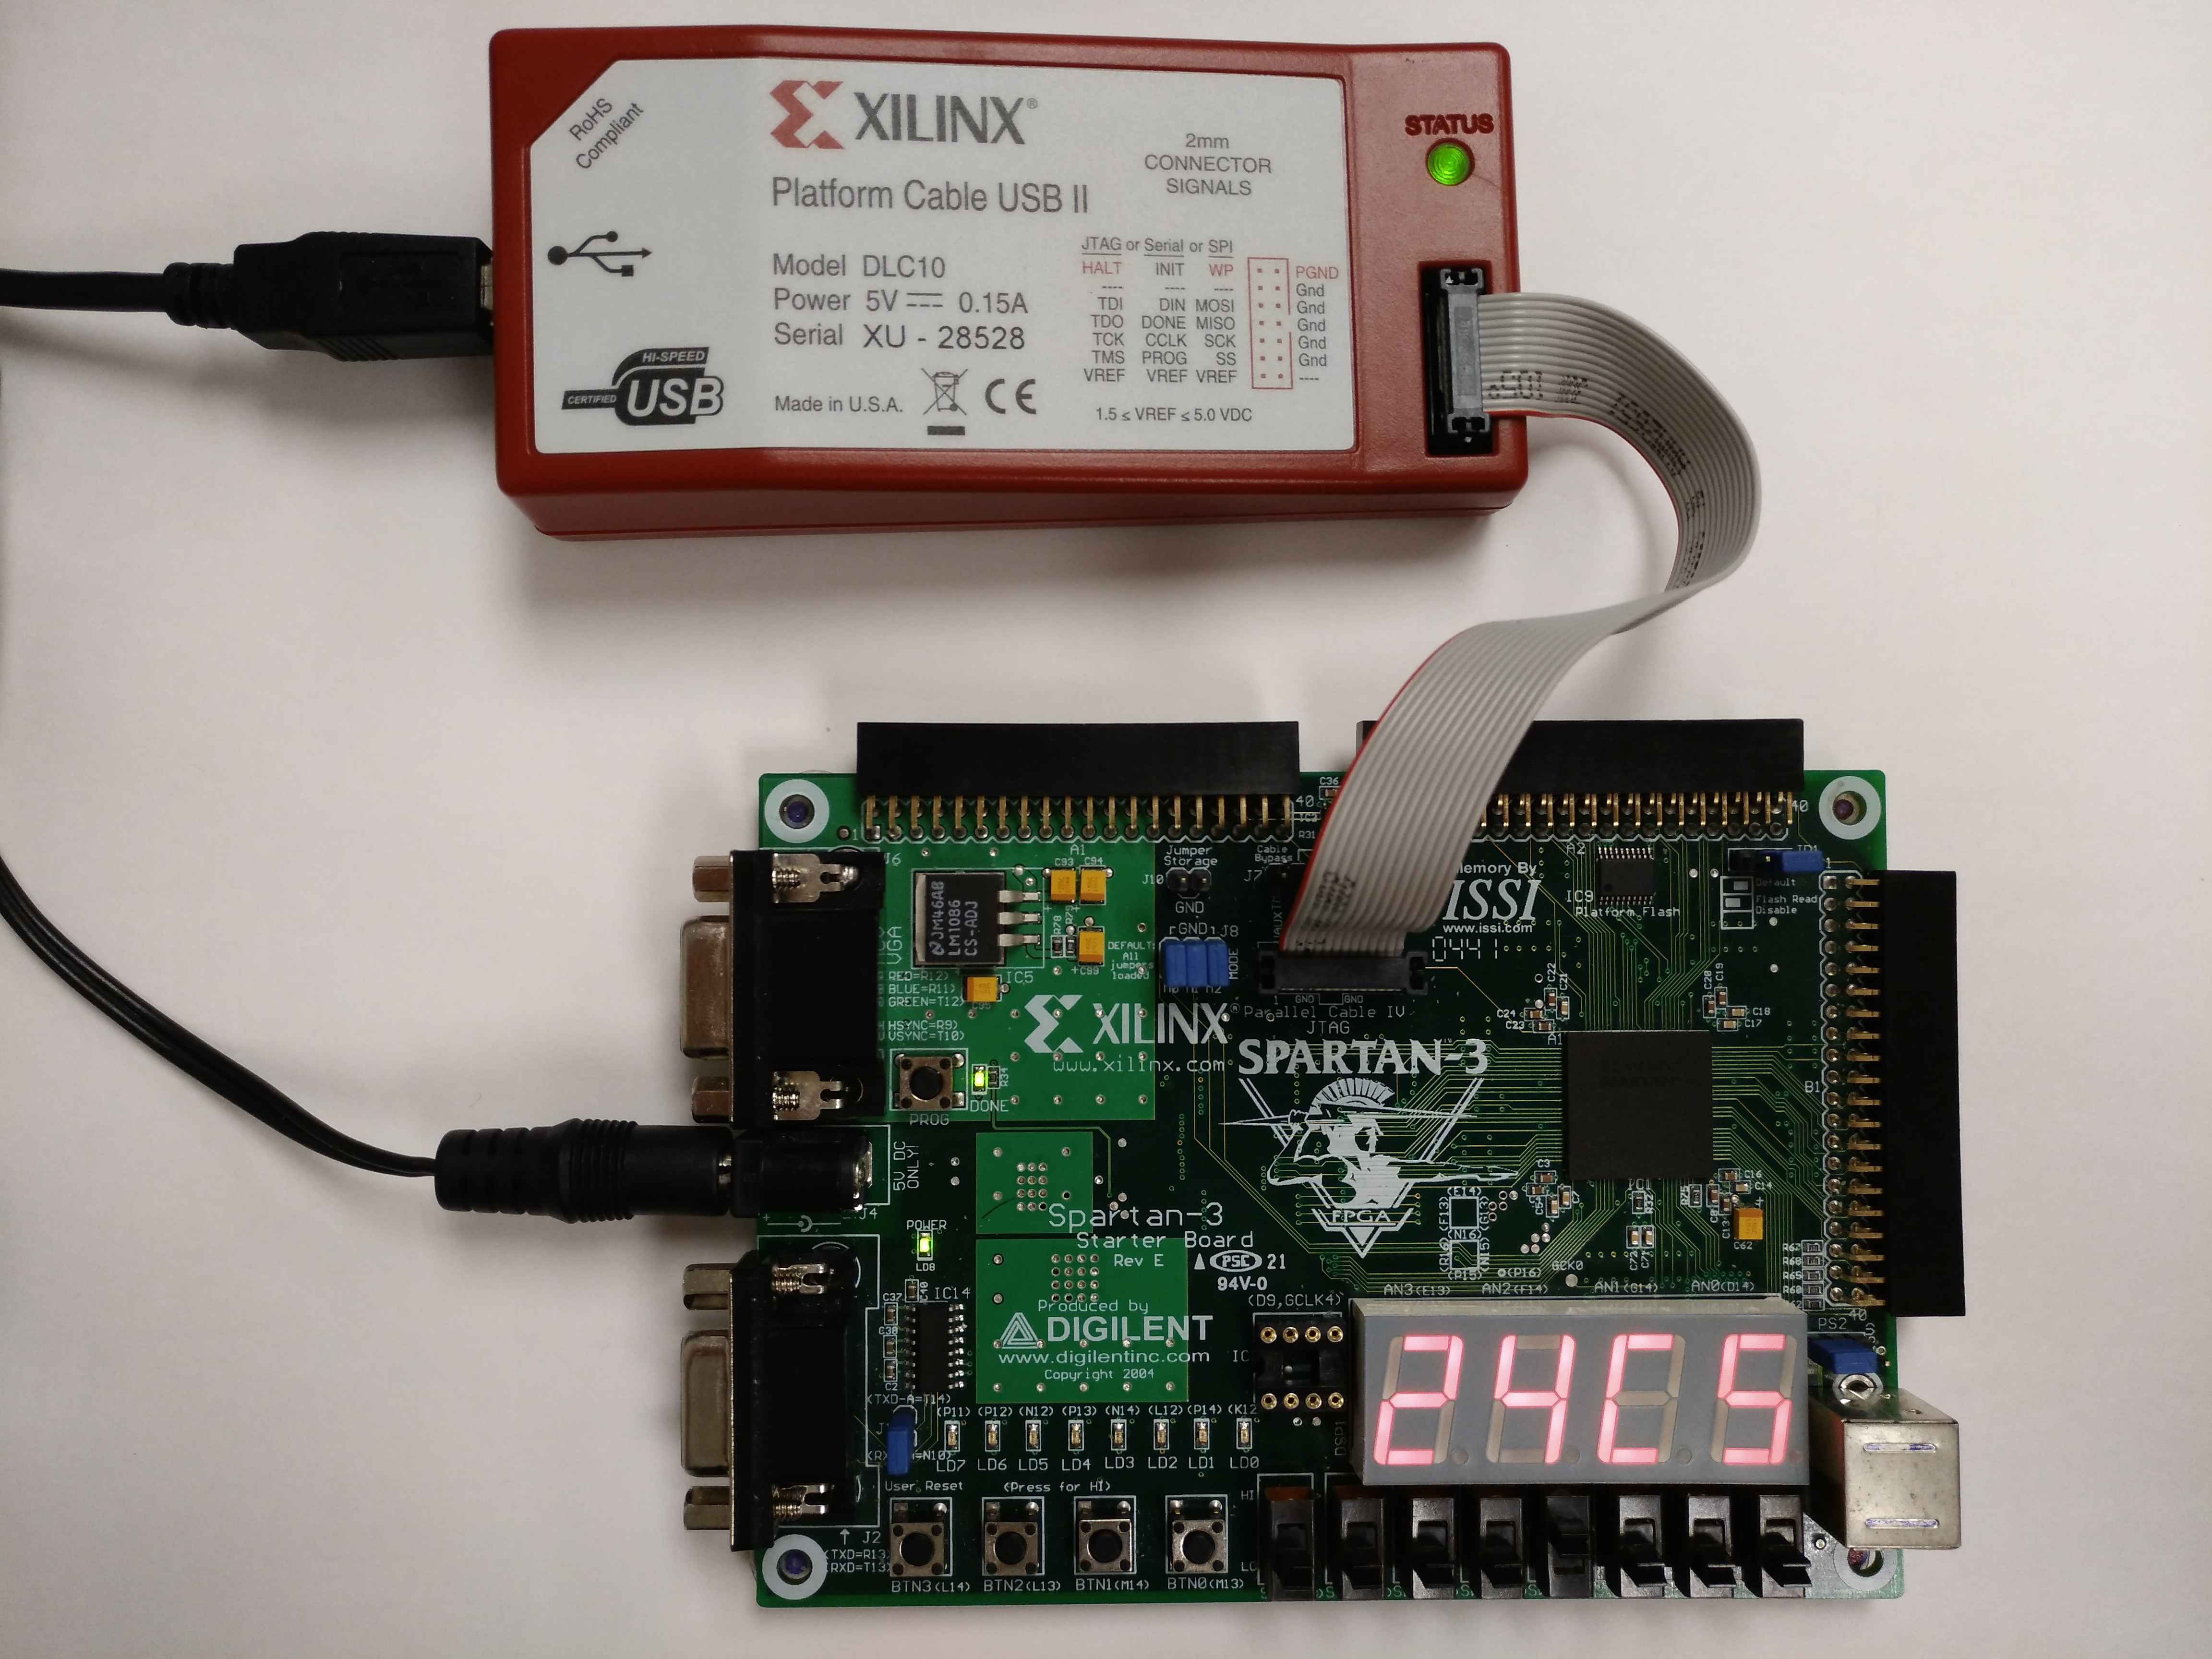
\includegraphics[width = 0.25\textwidth ]{CasoUso/5.jpg} & 5. & 
		  \includegraphics[width = 0.25\textwidth ]{CasoUso/6.jpg} & 6.  \\
		 \includegraphics[width = 0.25\textwidth ]{CasoUso/7.jpg} & 7. & 
		  \includegraphics[width = 0.25\textwidth ]{CasoUso/8.jpg} & 8.  \\
		 \includegraphics[width = 0.25\textwidth ]{CasoUso/9.jpg} & 9. & 
		  \includegraphics[width = 0.25\textwidth ]{CasoUso/10.jpg} & 10.  \\
		 \includegraphics[width = 0.25\textwidth ]{CasoUso/11.jpg} & 11. & 
		  \includegraphics[width = 0.25\textwidth ]{CasoUso/12.jpg} & 12.  \\
		 \includegraphics[width = 0.25\textwidth ]{CasoUso/13.jpg} & 13. & 
		  \includegraphics[width = 0.25\textwidth ]{CasoUso/14.jpg} & 14.  \\
	\end{longtable}